\documentclass[a4paper]{book}
\usepackage[
	%urlbordercolor = {1 1 1},
	%linkbordercolor = {1 1 1},
	%citebordercolor = {1 1 1},
	urlcolor = blue,
	colorlinks = true,
	citecolor = black,
	linkcolor = black]{hyperref}
\usepackage{graphicx}
\usepackage{xltxtra}
\usepackage{fancyhdr}
\usepackage{booktabs}
\usepackage{indentfirst}
\usepackage{framed,color}
\usepackage{array}
\usepackage[font=small,format=plain,labelfont=bf,up,textfont=it,up]{caption}

\definecolor{shadecolor}{gray}{0.90}

\setromanfont[Mapping=tex-text,Bold={* Bold}]{Ubuntu}
\setmonofont{DejaVu Sans Mono}

\XeTeXlinebreaklocale{en}


\settowidth{\parindent}{\qquad}

\title{Jasig CAS Server Manual}
\author{Jasig}

\makeatletter
\let\savedauthor=\@author
\let\savedtitle=\@title
\def\imgwidth{.6\linewidth}
\def\maxwidth{\ifdim\Gin@nat@width>\imgwidth\imgwidth
\else\Gin@nat@width\fi}
\makeatother

\title{\textbf{\savedtitle}}
\author{\textbf{\savedauthor}\thanks{This is the PDF file for the CAS Server Manual book contents. It is licensed under the Apache 2.0 license.}}
\def\w3cdtfymd{\the\year-\ifnum\month<10 0\fi\the\month-\ifnum\day<10 0\fi\the\day}
\date{\w3cdtfymd}
\renewcommand{\thefootnote}{\fnsymbol{footnote}}

\newcommand{\PreserveBackslash}[1]{\let\temp=\\#1\let\\=\temp}
\let\PBS=\PreserveBackslash
\makeatletter
  \setlength\headheight{12\p@}
  \setlength\headsep   {.25in}
  \setlength\topskip   {10\p@}
  \setlength\footskip{.35in}
  \setlength\textwidth{400\p@}
  
  \setlength\@tempdima{\paperheight}
  \addtolength\@tempdima{-2in}
  \divide\@tempdima\baselineskip
  \@tempcnta=\@tempdima
  \setlength\textheight{\@tempcnta\baselineskip}
  \addtolength\textheight{\topskip}
  
  \setlength\@tempdima        {\paperwidth}
  \addtolength\@tempdima      {-\textwidth}
  \setlength\oddsidemargin    {\paperwidth}
  \addtolength\oddsidemargin  {-2.35in}
  \addtolength\oddsidemargin  {-\textwidth}
  \setlength\marginparwidth   {0pt}
  \@settopoint\oddsidemargin
  \@settopoint\marginparwidth
  \setlength\evensidemargin  {\paperwidth}
  \addtolength\evensidemargin{-2.35in}
  \addtolength\evensidemargin{-\textwidth}
  \@settopoint\evensidemargin
  
  \setlength\topmargin{\paperheight}
  \addtolength\topmargin{-2in}
  \addtolength\topmargin{-\headheight}
  \addtolength\topmargin{-\headsep}
  \addtolength\topmargin{-\textheight}
  \addtolength\topmargin{-\footskip}     % this might be wrong!
  \addtolength\topmargin{-.5\topmargin}
  \@settopoint\topmargin
\makeatother

\fancypagestyle{plain}{\fancyhf{}\fancyfoot[LE,RO]{\footnotesize\textbf\thepage}}
\pagestyle{plain}

\renewcommand{\headrulewidth}{0pt}
\renewcommand{\footrulewidth}{0pt}

\newcounter{img}[chapter]
\renewcommand{\theimg}{\thechapter.\arabic{img}}
\newcommand{\img}[1]{\begin{figure}[h!]
	\refstepcounter{img}
	\label{img:\theimg}
	\centering\includegraphics[width=\maxwidth]{figures/\theimg.png}
	\caption{#1}
\end{figure}}

\newcounter{tab}[chapter]
\renewcommand{\thetab}{\thechapter.\arabic{tab}}

\newcommand{\prechap}{Chapter }
\newcommand{\postchap}{}
\newcommand{\presect}{Section }
\newcommand{\postsect}{}
\renewcommand{\chaptermark}[1]{\markboth{\textbf{\prechap \thechapter \postchap}\hspace*{1ex}#1}{}}
\renewcommand{\sectionmark}[1]{\markright{\textbf{\presect \thesection \postsect}\hspace*{1ex}#1}}
\newcommand{\chap}[1]{\newpage\thispagestyle{empty}\chapter{#1}\label{chap:\thechapter}}
\newcommand{\chapref}[1]{\hyperref[chap:#1]{\prechap #1\postchap}}
\newcommand{\imgref}[1]{\hyperref[img:#1]{Figure #1}}
\newcommand{\tabref}[1]{\hyperref[tab:#1]{Table #1}}
\newcommand{\e}[1]{$ \times 10^{#1}$}
\renewcommand{\contentsname}{Contents}
\renewcommand{\figurename}{Figure }
\renewcommand{\tablename}{Table }

\makeatletter
\def\@makechapterhead#1{%
  \vspace*{50\p@}%
  {\parindent \z@ \raggedright \normalfont
    \ifnum \c@secnumdepth >\m@ne
      \if@mainmatter
        \huge\bfseries \prechap \thechapter \postchap
        \par\nobreak
        \vskip 20\p@
      \fi
    \fi
    \interlinepenalty\@M
    \Huge \bfseries #1\par\nobreak
    \vskip 40\p@
  }}
\makeatother

\linespread{1.3}

\begin{document}
\frontmatter
\maketitle
\thispagestyle{empty}
\setcounter{tocdepth}{4}
\tableofcontents\newpage\thispagestyle{empty}

\mainmatter
\fancyhf{}
\fancyhead[LE]{{\small\leftmark}}
\fancyhead[RO]{{\small\rightmark}}
\fancyhead[RE,LO]{{\small\savedauthor\hspace*{1ex}\textbf{\savedtitle}}}
\fancyfoot[LE,RO]{\small\textbf\thepage}
\pagestyle{fancy}

\chap{What is Jasig CAS?}

\begin{figure}[htb]
\centering
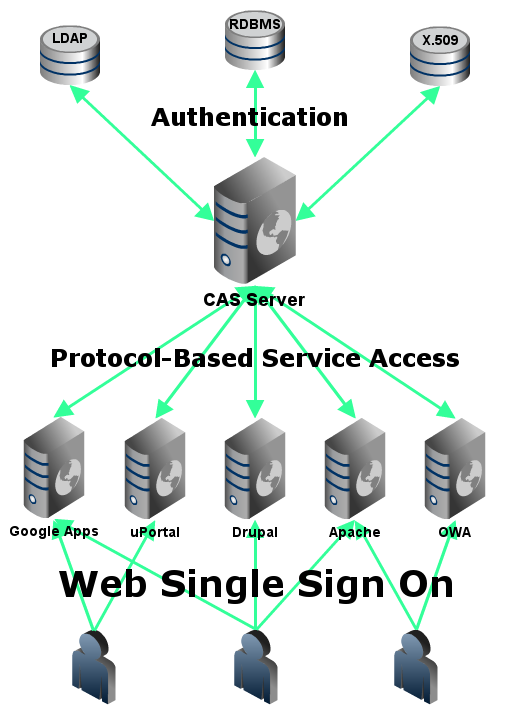
\includegraphics{media/sso-diagram.png}
\caption{Big picture diagram}
\end{figure}

CAS is a multiprotocol Web single sign-on (SSO) product composed of a single logical server component that services authentication requests from multiple CAS clients that communicate via one or more supported protocols. The CAS server delegates authentication decisions to any number of supported authentication mechanisms including LDAP/Active Directory, Kerberos, and RDBMS. The hallmark of CAS is ease of integration and extension in support of a wide variety of environments. In addition to supporting a large number of technologies out of the box, the well-documented API extension points have enabled deployers to develop custom components to support novel use cases not supported by default.

\section{Features}

CAS has a number of features that distinguish it from other SSO products:

\subsection{Single Sign-On (SSO) Implementation}

Unlike many SSO products, CAS does not use shared cookies to authenticate to services within the SSO domain. The CAS implementation uses a secure SSO session identifier (ticket-granting ticket in CAS protocol parlance), shared exclusively with the CAS server, to generate one-time-use credentials (service tickets in CAS protocol parlance) that are used to access services within the SSO domain. Passing the “master key” session identifier exclusively between the user's browser and CAS server dramatically limits the potential for man-in-the-middle attacks on the session identifier. CAS benefits from increased security in this regard over shared cookie strategies.

\subsection{Integration}

CAS client integration components are available for all popular Web development frameworks and many popular Web applications.

\subsubsection{Popular CAS Clients}

\begin{itemize}
\item
  Java
\item
  Microsoft .NET Framework
\item
  PHP
\item
  Outlook Web Access
\item
  Drupal
\item
  Confluence
\end{itemize}
The combination of open protocols and open source facilitate the development of integration components for almost any product as has been demonstrated over many years by the development of components for frameworks as varied as PL/SQL and Cold Fusion.

\subsection{Authentication Providers}

The CAS server authenticates users by means of the AuthenticationHandler component for which a number of implementations are provided with the CAS distribution.

\subsubsection{Bundled Authentication Providers}

\begin{itemize}
\item
  LDAP (e.g. Active Directory, OpenLDAP)
\item
  RDBMS
\item
  SPNEGO
\item
  X.509/Client SSL
\item
  JAAS
\item
  RADIUS
\item
  Flat file
\end{itemize}
CAS has a proven track record of supporting custom authentication providers such as proprietary Web services. Adopters leverage the open and well-documented source to develop custom AuthenticationHandler components and wire them into the application using Spring XML configuration. The result is straightforward extension for virtually any authentication need.

\subsection{Authorization}

CAS approaches authorization from the perspective that authorization is the responsibility of individual services that authenticate to CAS. This design owes to the history of CAS having been developed in the Higher Education setting, which is typically highly decentralized and ill suited to agreement and enforcement of centralized authorization policy. CAS supports decentralized authorization via an attribute release mechanism where any number of stores may be configured to load and store attributes about principals upon authentication to CAS, and which are released to services when they authenticate to CAS. Attributes are interpreted by services as needed, commonly for authorization and personalization.

\section{Support}

CAS is supported by a community of developers and users via a variety of means.

\subsection{Community Support Channels}

\begin{itemize}
\item
  Product documentation (like this manual)
\item
  Real-time user support via the \href{mailto:cas-user@lists.jasig.org}{\texttt{cas-user@lists.jasig.org}} mailing list
\item
  Discussion via Internet Relay Chat (IRC) in the \#jasig-cas channel on irc.freenode.net . Note that while several CAS developers and adopters typically hang out in this IRC chat room, the project has no commitment to 24x7 support via that mechanism and you may be better off directing your question to the cas-user@ email list.
\item
  Conferences and webinars
\end{itemize}
\subsection{Commercial Support Channels}

In addition to community support, the Jasig CAS project has a \href{http://www.jasig.org/cas/support/solutions-providers}{CAS Solutions Providers} program for recognizing vendors and consultants that provide services related to Jasig CAS. Please note that acceptance in the Solution Provider Program does not constitute an endorsement or recommendation by Jasig.

Current CAS Solution Provider:

\begin{itemize}
\item
  \href{http://www.unicon.net/}{Unicon Inc.} (a \href{http://www.jasig.org/jasig-membership-partners}{Jasig Partner}) \href{http://www.unicon.net/services/cas/support}{Cooperative Support for CAS} and \href{http://www.unicon.net/services/cas}{consulting services related to CAS}.
\end{itemize}

\end{document}
